\chapter{Immersions and Submersions}\label{chap7}

\section*{Immersions and Submanifolds}

Let $f:N\to M$ be a smooth map. We say that $f$ is an {\em immersion} at a point $b\in N$ if the tangent map $T_{b}(f):T_{b}(N)\to T_{f(b)}(M)$ is injective.\pageoriginale We say that $f$ is an immersion if $f$ is injective at every point of $N$. We have

\begin{theorem}\label{chap7-thm7.1}
Let $n=\dim M$ and $p=\dim N$. Let $f$ be an immersion at $b\in N$. Then there exists neighbourhoods $V$ of $b$, $U$ of $f(b)$ with $f(V)\subset U$ and a coordinate system $(x_{1},\ldots,x_{n})$ in $U$ with $x_{i}\circ f=0$ on $V$ for $p<i\leq n$ and such that $\{x_{i}\circ f\}$, $1\leq i\leq p$ give a coordinate system for $N$ in $V$.
\end{theorem}

Moreover if $T_{b}(f):T_{b}(N)\to T_{f(b)}(M)$ is an isomorphism there exists neighbourhoods $V$ of $b$ and $U$ of $f(b)$ such that $f(V)\subset U$ and $f|V\to U$ is a diffeomorphism (inverse function theorem).

Let $M$ be a manifold and $N$ a subset of $M$, with the following property: for every $b\in N$ there exists a neighbourhood $U$ of $b$ in $M$ and a coordinate system $(x_{1},\ldots,x_{n})$ in $U$ (for $M$) and in integer $p\leq n$ (depending only on $N$) such that $N\cap U$ is given by $x_{i}=0$ for $p<i\leq n$. Then $N$ has a natural structure of a $p$-dimensional manifold such that the functions $\left\{x_{i}|_{N\cap U}\right\}_{1\leq i\leq p}$ form a coordinate system for $N$ in $N\cap U$. ($N$ is provided with the topology induced from $M$). We then say that $N$ is a submanifold of $M$. If moreover $N$ is a closed subset of $M$ we say that $N$ is a closed submanifold.

\begin{remarks*}
\begin{itemize}
\item[(1)] If $f:N\to M$ is an immersion such that $f$ is a homeomorphism of $N$ onto $f(N)$, then $f(N)$ is a submanifold and $f:N\to f(N)$ is a diffeomrophism. In this case we say that $f$ is an imbedding.

\item[(2)] If $f:N\to M$ is an injective immersion, $f(N)$ need not be a submanifold of $M$.
\begin{figure}[H]
\centering
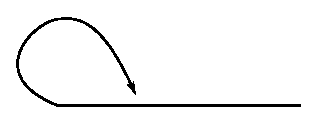
\includegraphics{1.eps}
\end{figure}\pageoriginale
The line approaches itself without touching.
\end{itemize}
\end{remarks*}

\section*{Submersions}

Let $f:M\to N$ be a smooth map. We say that $f$ is a submersion at a point $a\in M$ if $T_{a}(f):T_{a}(M)\to T_{f(a)}(N)$ is surjective. The map $f$ is said to be a submersion if it is a submersion at every point of $M$.

\subsection*{Theorem (Implicit function theorem) \thnum{7.2}.\label{chap7-thm7.2}}

Let $f:M\to N$ be a submersion at $a\in M$. (Let $n=\dim M$ and $q=\dim N$). There exists charts $(U,\phi)$, $(V,\psi)$ for respectively $M$ and $N$, with $a\in U$, $f(a)\in V$, $f(U)\subset V$, $\varphi(a)=0\in \mathbb{R}^{n}$, $\psi\circ f(a)=0\in \mathbb{R}^{q}$ with commutativity in the diagram
\[
\xymatrix@=1.2cm{
U\ar[d]^{\phi}\ar[r]^{f} & V\ar[d]^{\psi}\\
\varphi(U)\ar[r]_{F} & \psi(V)
}
\]
where $F$ is (the restriction of) the map 
$$
\mathbb{R}^{n}\to \mathbb{R}^{q}(x_{1},\ldots,x_{n})\mapsto (x_{1},\ldots,x_{q}).
$$

It follows that a submersion is an open map.



